\section{Ход работы}
\subsection{Измерения}

1. Проверена целостность установки на рисунке 1.
\begin{figure}[H]
    \centering
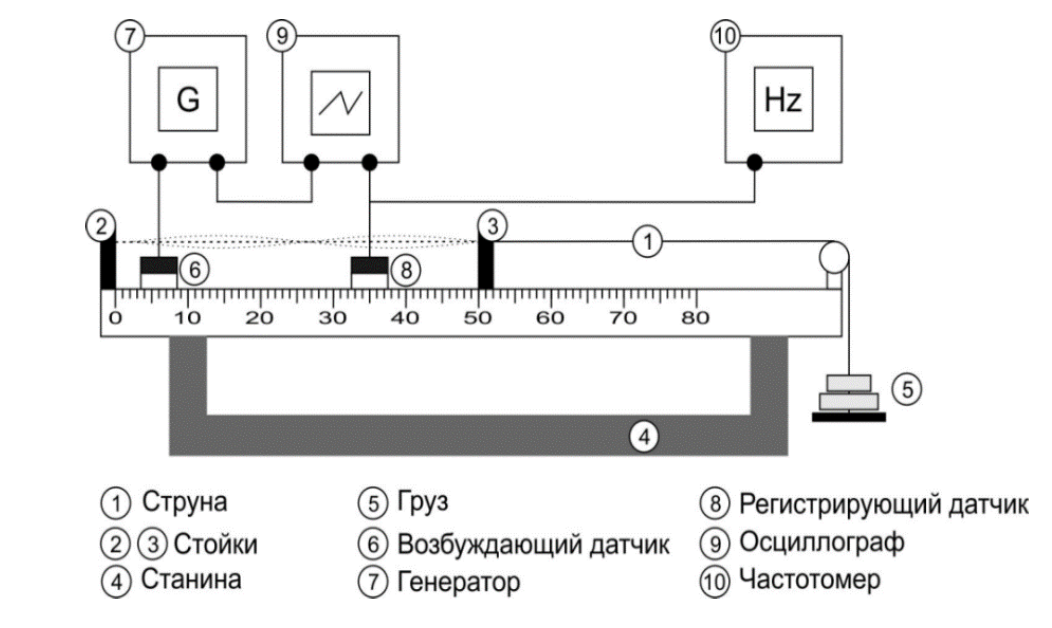
\includegraphics[width=1.\linewidth,center]{p 1.png}
    \caption{Установка}
    \label{fig:my_label}
\end{figure}

2. Установлено начальное значение длины струны $L = 50$ см. Погонная плотность струны $\rho_l = 568,4$ мг/м.

3. На платформу поставлены грузы общей массой $m_1 = 1020,4$ г.

4. Оценены скорость распространения ( в м/с ) и частота основной гармоники ( в Гц ).
\[u_1 = \sqrt{\frac{mg}{l}} = 132,7\]
\[\nu_1 = \frac{1}{2L}u = 132,7\]

5. Эксперементальным путём в ходе измерений на осциллографе получены значения для 7 гармоник:
\[\nu_{11} = 132,5\]
\[\nu_{12} = 267\]
\[\nu_{13} = 398\]
\[\nu_{14} = 537\]
\[\nu_{15} = 670\]
\[\nu_{16} = 808\]
\[\nu_{17} = 944\]

Аналогичные эксперименты и расчеты проведены еще для 3 наборов.

6. 2 набор ( $m_2 = 569,5$ г, $u_2 = 95,1$ м/с, $\nu_2 = 95,1$ Гц ):
\[\nu_{21} = 101,6\]
\[\nu_{22} = 204\]
\[\nu_{23} = 209\]
\[\nu_{24} = 411\]
\[\nu_{25} = 517\]
\[\nu_{26} = 630\]
\[\nu_{27} = 729\]

7. 3 набор ( $m_3 = 1483,4$ г, $u_2 = 160,0$ м/с, $\nu_2 = 160,0$ Гц ):
\[\nu_{31} = 158,7\]
\[\nu_{32} = 326\]
\[\nu_{33} = 486\]
\[\nu_{34} = 648\]
\[\nu_{35} = 754\]
\[\nu_{36} = 986\]
\[\nu_{37} = 1210\]

8. 4 набор ( $m_4 = 1994,3$ г, $u_2 = 185,5$ м/с, $\nu_2 = 185,5$ Гц ):
\[\nu_{41} = 177,9\]
\[\nu_{42} = 361\]
\[\nu_{43} = 542\]
\[\nu_{44} = 723\]
\[\nu_{45} = 906\]
\[\nu_{46} = 1087\]
\[\nu_{47} = 1270\]
\subsection{Обработка данных}

9. Построены графики зависимостей частоты $\nu_n$ от номера $n$ гармоники для различных натяжений $T$.
\begin{figure}[H]
    \centering
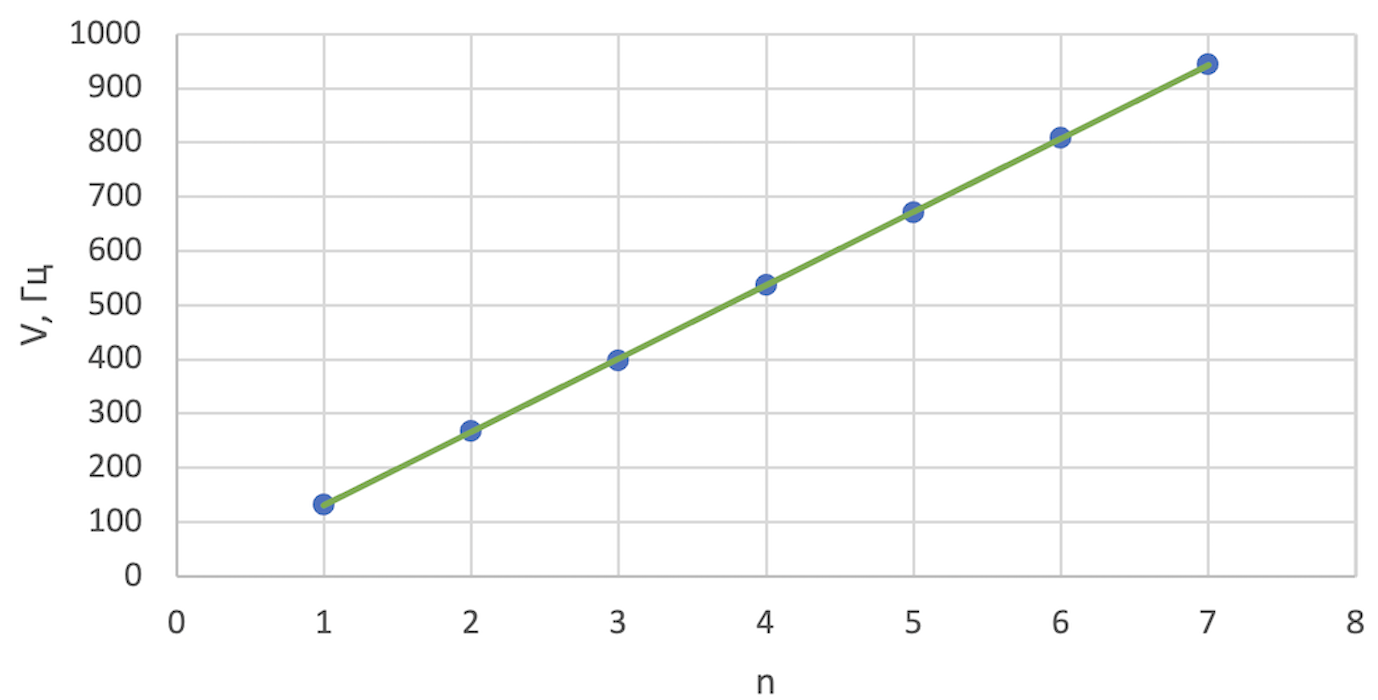
\includegraphics[width=1.\linewidth,center]{p 2.png}
    \caption{1 набор}
    \label{fig:my_label}
\end{figure}
\begin{figure}[H]
    \centering
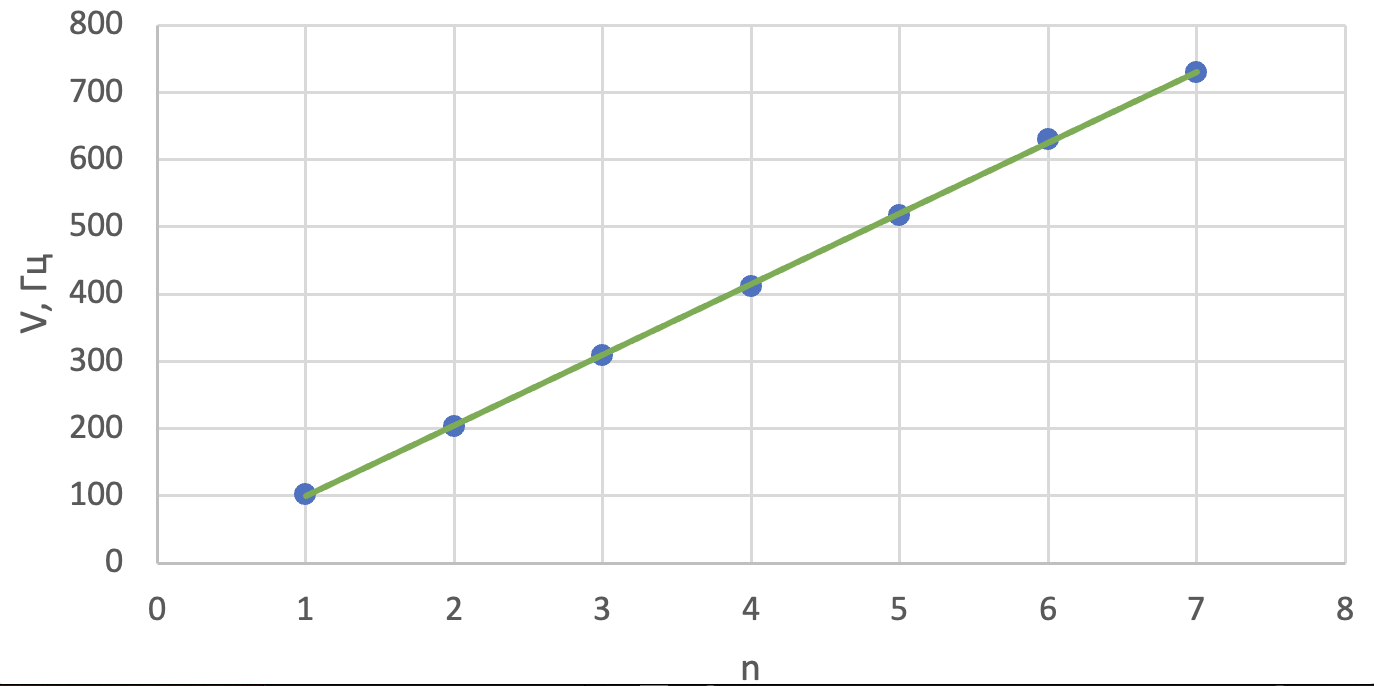
\includegraphics[width=1.\linewidth,center]{p 3.png}
    \caption{2 набор}
    \label{fig:my_label}
\end{figure}
\begin{figure}[H]
    \centering
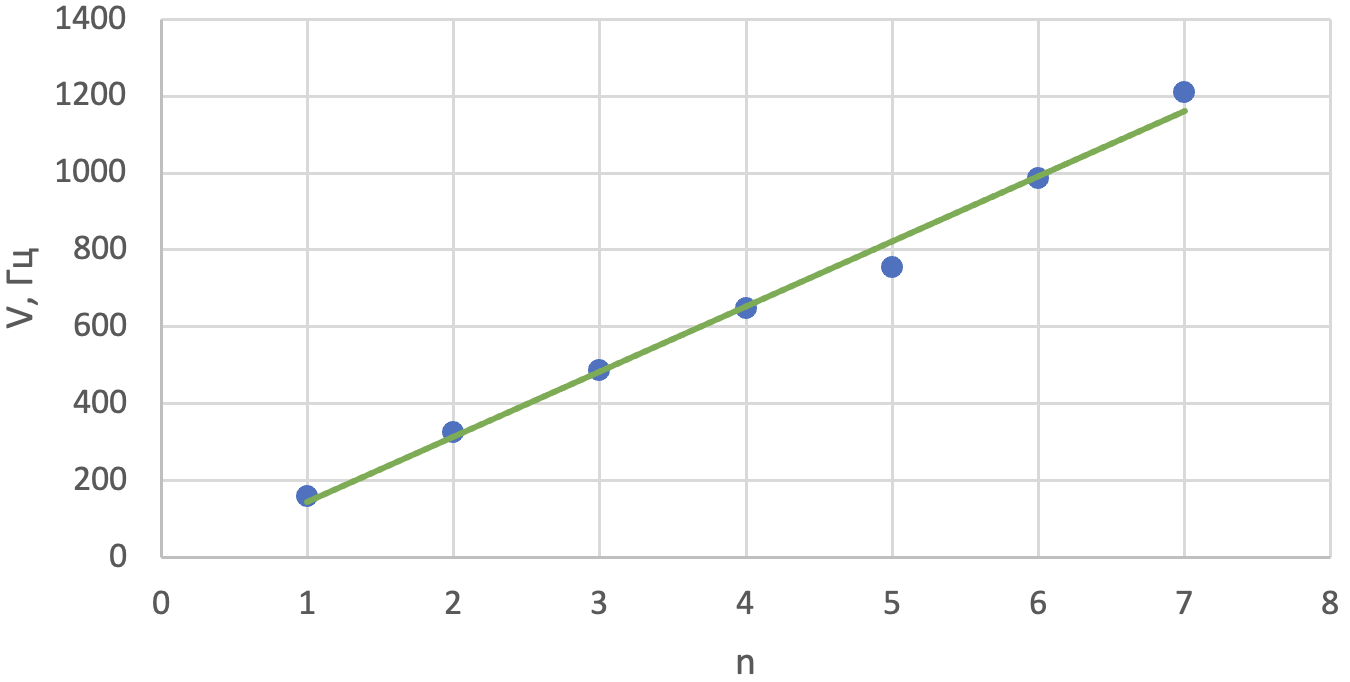
\includegraphics[width=1.\linewidth,center]{p 4.png}
    \caption{3 набор}
    \label{fig:my_label}
\end{figure}
\begin{figure}[H]
    \centering
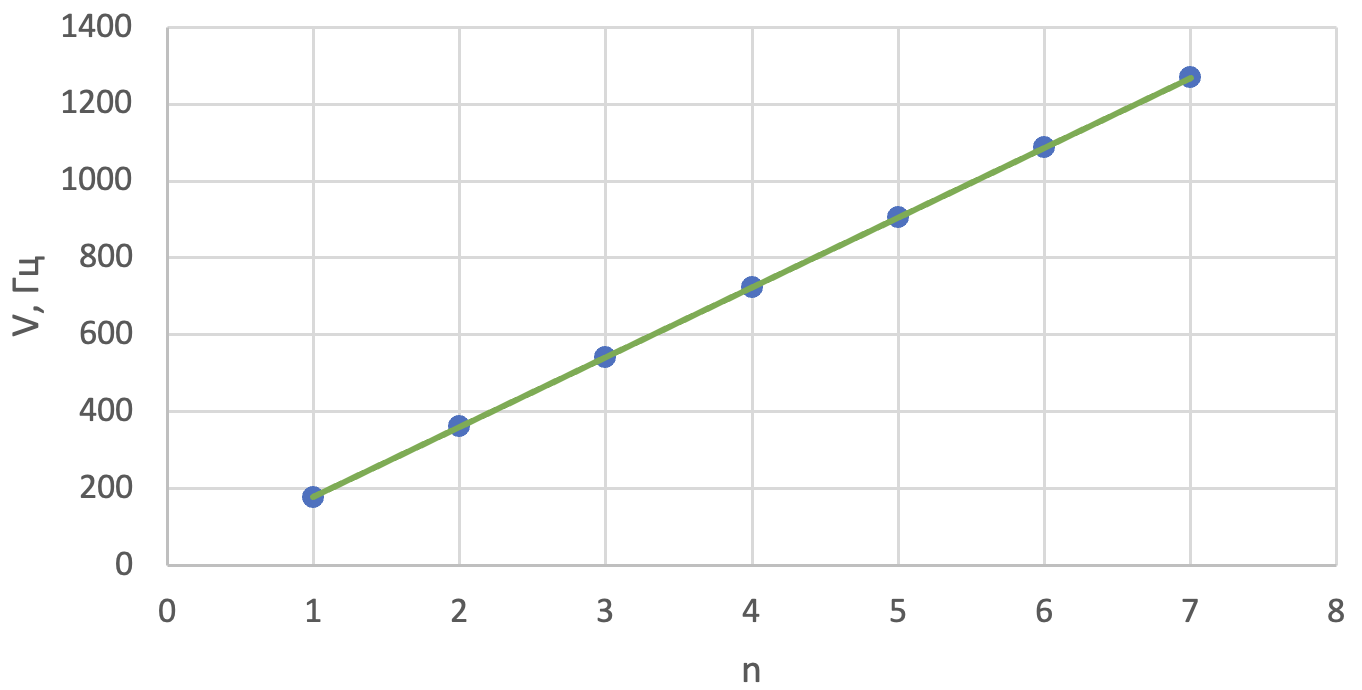
\includegraphics[width=1.\linewidth,center]{p 5.png}
    \caption{4 набор}
    \label{fig:my_label}
\end{figure}

10. Посчитаем скорости, получившиеся эксперементально по наклону:
\[u = 2L\frac\nu n\]
\[u_1 = 135,3\]
\[u_2 = 105,1\]
\[u_3 = 169,3\]
\[u_4 = 181,8\]

11. Построим график зависимости $u^2\left(T\right)$:
\begin{figure}[H]
    \centering
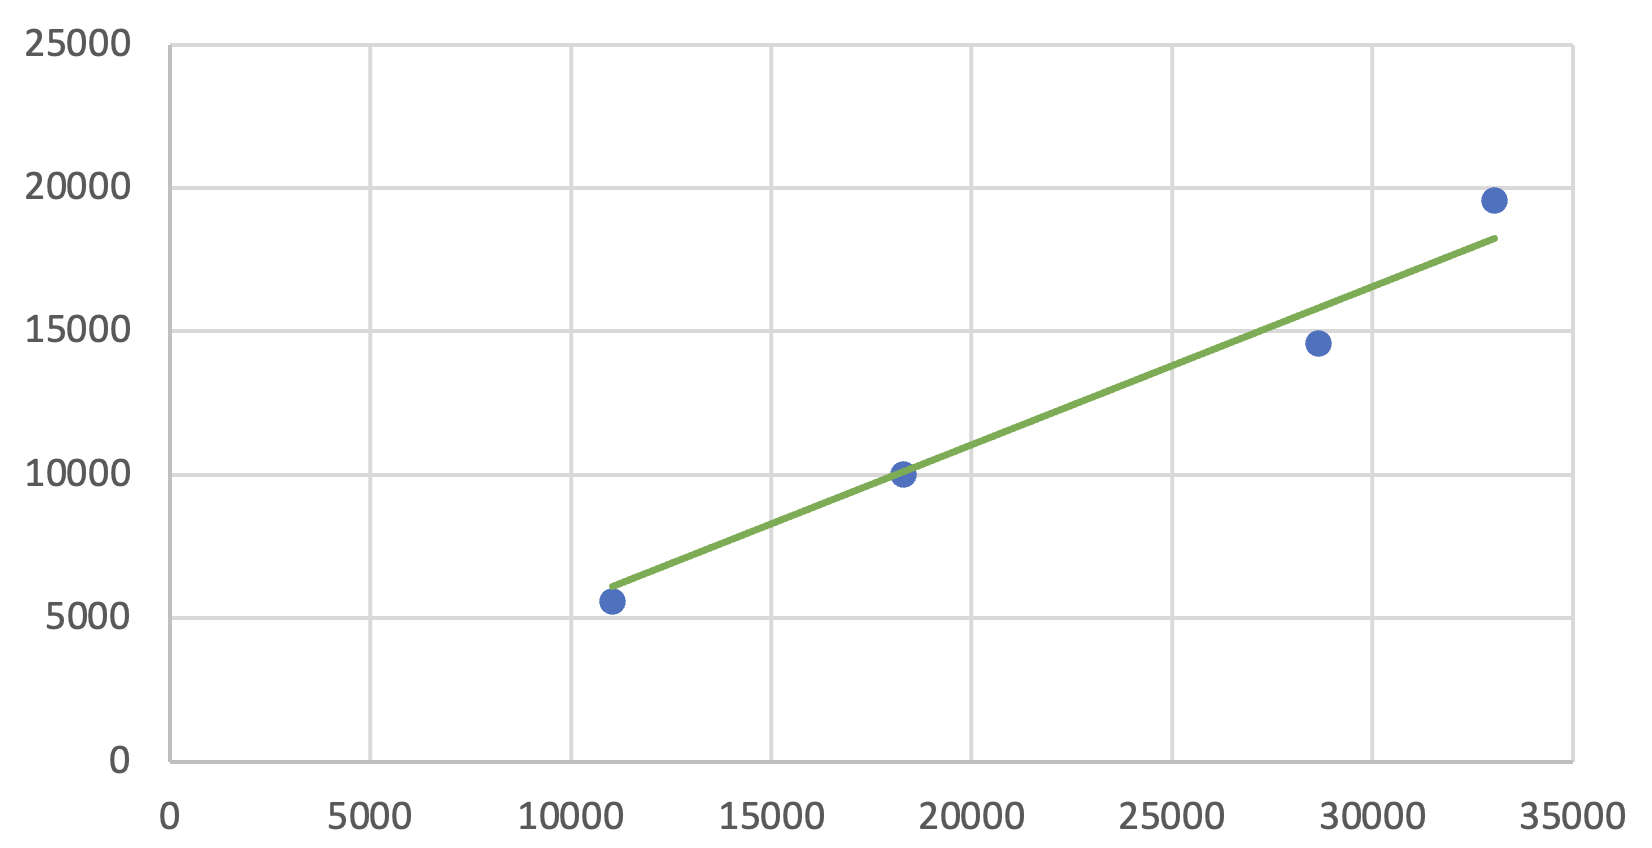
\includegraphics[width=1.\linewidth,center]{p 6.png}
    \caption{}
    \label{fig:my_label}
\end{figure}

13. Посчитаем по углу наклона $\rho_l$:
\[\rho_l = 593,9 \frac{mg}{m}.\]

14. По методу наименьших квадратов посчитаем погрешность:
\[\Delta\rho_l = \sqrt{\frac{1}{3\cdot4}\left(\left(\rho_1 - \rho_l\right)^2+\dots\right)} = 38\]

15. Итоговый результат для $\rho_l$:
\[\rho_l = \left(594 \pm 38\right) \frac{mg}{m}\]

\subsection{АЧХ}

16. Построим график ( рисунок 7 ). Посчитаем добротность струны по формуле:
\[Q = \frac{\nu}{\Delta\nu} = 593\]

\begin{figure}[H]
    \centering
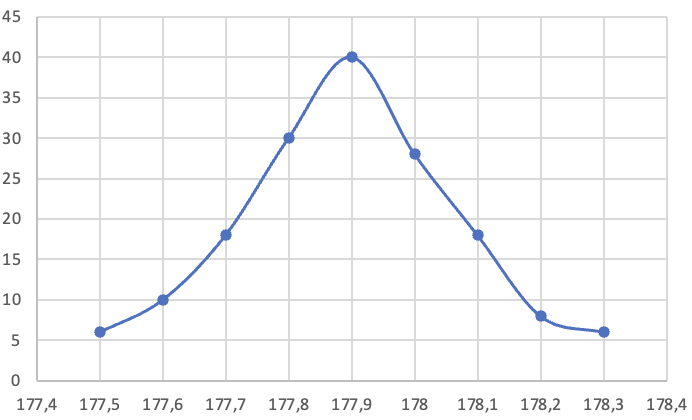
\includegraphics[width=1.\linewidth,center]{p 7.png}
    \caption{}
    \label{fig:my_label}
\end{figure}
